Considerar $N$ puntos dados en un plano, y el objetivo es generar una envolvente convexa, es decir, el polígono convexo más pequeño que contiene todos los puntos dados. En la siguientes figuras se observa el caso que queremos presentar. La izquierda se presenta el grupo de puntos mientras en la derecha se presenta el mismo grupo de puntos pero con aquellos que fueron seleccionados que formarían parte del polígono convexo o envolvente convexa.

\begin{figure}[!h]
	\centering
	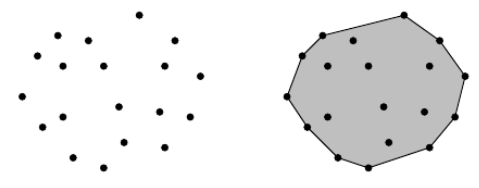
\includegraphics[scale=0.4]{img/cubierta_convexa}
	\label{fig:cubiertaconvexa}
\end{figure}

El problema (planar) de la cubierta convexa se define de la siguiente forma: Dado un conjunto P de n puntos en el plano, calcular la representación del polígono convexo cerrado que representa la cubierta convexa de P. La representación más simple de una cubierta convexa es la enumeración en el sentido inverso a las manecillas del reloj de sus vértices. Idealmente la cubierta convexa debe consistir sólo de los puntos extremos, en el sentido que si tres puntos caen en un vértice de la frontera de la cubierta convexa, entonces el punto medio no debe ser tomado en cuenta como parte de la cubierta. 

\begin{figure}[h]
	\centering
	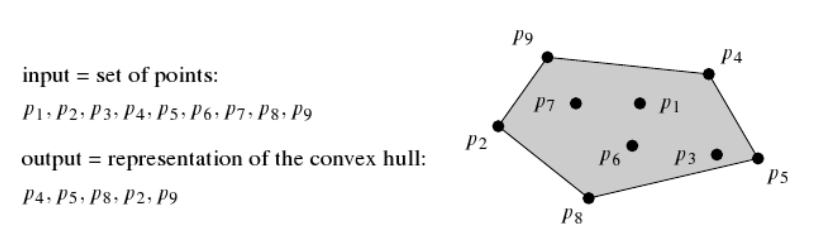
\includegraphics[scale=0.35]{img/cubierta_convexa2}
\end{figure}